% Options for packages loaded elsewhere
\PassOptionsToPackage{unicode}{hyperref}
\PassOptionsToPackage{hyphens}{url}
%
\documentclass[
  spanish,
]{article}
\usepackage{lmodern}
\usepackage{amssymb,amsmath}
\usepackage{ifxetex,ifluatex}
\ifnum 0\ifxetex 1\fi\ifluatex 1\fi=0 % if pdftex
  \usepackage[T1]{fontenc}
  \usepackage[utf8]{inputenc}
  \usepackage{textcomp} % provide euro and other symbols
\else % if luatex or xetex
  \usepackage{unicode-math}
  \defaultfontfeatures{Scale=MatchLowercase}
  \defaultfontfeatures[\rmfamily]{Ligatures=TeX,Scale=1}
\fi
% Use upquote if available, for straight quotes in verbatim environments
\IfFileExists{upquote.sty}{\usepackage{upquote}}{}
\IfFileExists{microtype.sty}{% use microtype if available
  \usepackage[]{microtype}
  \UseMicrotypeSet[protrusion]{basicmath} % disable protrusion for tt fonts
}{}
\makeatletter
\@ifundefined{KOMAClassName}{% if non-KOMA class
  \IfFileExists{parskip.sty}{%
    \usepackage{parskip}
  }{% else
    \setlength{\parindent}{0pt}
    \setlength{\parskip}{6pt plus 2pt minus 1pt}}
}{% if KOMA class
  \KOMAoptions{parskip=half}}
\makeatother
\usepackage{xcolor}
\IfFileExists{xurl.sty}{\usepackage{xurl}}{} % add URL line breaks if available
\IfFileExists{bookmark.sty}{\usepackage{bookmark}}{\usepackage{hyperref}}
\hypersetup{
  pdflang={es},
  hidelinks,
  pdfcreator={LaTeX via pandoc}}
\urlstyle{same} % disable monospaced font for URLs
\usepackage{color}
\usepackage{fancyvrb}
\newcommand{\VerbBar}{|}
\newcommand{\VERB}{\Verb[commandchars=\\\{\}]}
\DefineVerbatimEnvironment{Highlighting}{Verbatim}{commandchars=\\\{\}}
% Add ',fontsize=\small' for more characters per line
\newenvironment{Shaded}{}{}
\newcommand{\AlertTok}[1]{\textcolor[rgb]{1.00,0.00,0.00}{\textbf{#1}}}
\newcommand{\AnnotationTok}[1]{\textcolor[rgb]{0.38,0.63,0.69}{\textbf{\textit{#1}}}}
\newcommand{\AttributeTok}[1]{\textcolor[rgb]{0.49,0.56,0.16}{#1}}
\newcommand{\BaseNTok}[1]{\textcolor[rgb]{0.25,0.63,0.44}{#1}}
\newcommand{\BuiltInTok}[1]{#1}
\newcommand{\CharTok}[1]{\textcolor[rgb]{0.25,0.44,0.63}{#1}}
\newcommand{\CommentTok}[1]{\textcolor[rgb]{0.38,0.63,0.69}{\textit{#1}}}
\newcommand{\CommentVarTok}[1]{\textcolor[rgb]{0.38,0.63,0.69}{\textbf{\textit{#1}}}}
\newcommand{\ConstantTok}[1]{\textcolor[rgb]{0.53,0.00,0.00}{#1}}
\newcommand{\ControlFlowTok}[1]{\textcolor[rgb]{0.00,0.44,0.13}{\textbf{#1}}}
\newcommand{\DataTypeTok}[1]{\textcolor[rgb]{0.56,0.13,0.00}{#1}}
\newcommand{\DecValTok}[1]{\textcolor[rgb]{0.25,0.63,0.44}{#1}}
\newcommand{\DocumentationTok}[1]{\textcolor[rgb]{0.73,0.13,0.13}{\textit{#1}}}
\newcommand{\ErrorTok}[1]{\textcolor[rgb]{1.00,0.00,0.00}{\textbf{#1}}}
\newcommand{\ExtensionTok}[1]{#1}
\newcommand{\FloatTok}[1]{\textcolor[rgb]{0.25,0.63,0.44}{#1}}
\newcommand{\FunctionTok}[1]{\textcolor[rgb]{0.02,0.16,0.49}{#1}}
\newcommand{\ImportTok}[1]{#1}
\newcommand{\InformationTok}[1]{\textcolor[rgb]{0.38,0.63,0.69}{\textbf{\textit{#1}}}}
\newcommand{\KeywordTok}[1]{\textcolor[rgb]{0.00,0.44,0.13}{\textbf{#1}}}
\newcommand{\NormalTok}[1]{#1}
\newcommand{\OperatorTok}[1]{\textcolor[rgb]{0.40,0.40,0.40}{#1}}
\newcommand{\OtherTok}[1]{\textcolor[rgb]{0.00,0.44,0.13}{#1}}
\newcommand{\PreprocessorTok}[1]{\textcolor[rgb]{0.74,0.48,0.00}{#1}}
\newcommand{\RegionMarkerTok}[1]{#1}
\newcommand{\SpecialCharTok}[1]{\textcolor[rgb]{0.25,0.44,0.63}{#1}}
\newcommand{\SpecialStringTok}[1]{\textcolor[rgb]{0.73,0.40,0.53}{#1}}
\newcommand{\StringTok}[1]{\textcolor[rgb]{0.25,0.44,0.63}{#1}}
\newcommand{\VariableTok}[1]{\textcolor[rgb]{0.10,0.09,0.49}{#1}}
\newcommand{\VerbatimStringTok}[1]{\textcolor[rgb]{0.25,0.44,0.63}{#1}}
\newcommand{\WarningTok}[1]{\textcolor[rgb]{0.38,0.63,0.69}{\textbf{\textit{#1}}}}
\usepackage{longtable,booktabs}
% Correct order of tables after \paragraph or \subparagraph
\usepackage{etoolbox}
\makeatletter
\patchcmd\longtable{\par}{\if@noskipsec\mbox{}\fi\par}{}{}
\makeatother
% Allow footnotes in longtable head/foot
\IfFileExists{footnotehyper.sty}{\usepackage{footnotehyper}}{\usepackage{footnote}}
\makesavenoteenv{longtable}
\usepackage{graphicx}
\makeatletter
\def\maxwidth{\ifdim\Gin@nat@width>\linewidth\linewidth\else\Gin@nat@width\fi}
\def\maxheight{\ifdim\Gin@nat@height>\textheight\textheight\else\Gin@nat@height\fi}
\makeatother
% Scale images if necessary, so that they will not overflow the page
% margins by default, and it is still possible to overwrite the defaults
% using explicit options in \includegraphics[width, height, ...]{}
\setkeys{Gin}{width=\maxwidth,height=\maxheight,keepaspectratio}
% Set default figure placement to htbp
\makeatletter
\def\fps@figure{htbp}
\makeatother
\setlength{\emergencystretch}{3em} % prevent overfull lines
\providecommand{\tightlist}{%
  \setlength{\itemsep}{0pt}\setlength{\parskip}{0pt}}
\setcounter{secnumdepth}{-\maxdimen} % remove section numbering
\ifxetex
  % Load polyglossia as late as possible: uses bidi with RTL langages (e.g. Hebrew, Arabic)
  \usepackage{polyglossia}
  \setmainlanguage[]{spanish}
\else
  \usepackage[shorthands=off,main=spanish]{babel}
\fi

\author{}
\date{}

\begin{document}

\begin{Shaded}
\begin{Highlighting}[]
\FunctionTok{Campus}\KeywordTok{:}\AttributeTok{ Ciudad Universitaria}
\FunctionTok{Facultad}\KeywordTok{:}\AttributeTok{ Ingeniería}
\FunctionTok{Materia }\KeywordTok{:}\AttributeTok{ Inteligencia Artificial}
\FunctionTok{Semestre}\KeywordTok{:}\AttributeTok{ 2022{-}2}
\FunctionTok{Equipo}\KeywordTok{:}\AttributeTok{ }\DecValTok{1}
\FunctionTok{Clave}\KeywordTok{:}\AttributeTok{ }\DecValTok{0406}
\FunctionTok{Participantes}\KeywordTok{:}\AttributeTok{ }
\KeywordTok{{-}}\AttributeTok{ Barrera Peña Víctor Miguel}
\KeywordTok{{-}}\AttributeTok{ Espino De Horta Joaquín Gustavo}
\AttributeTok{    }
\FunctionTok{Profesor}\KeywordTok{:}\AttributeTok{ Dr. Ismael Everardo Barcenas Patiño}
\FunctionTok{Título }\KeywordTok{:}\AttributeTok{ Proyecto }
\FunctionTok{Subtítulo }\KeywordTok{:}\AttributeTok{ Inferencia bayesiana}
\FunctionTok{Fecha entrega}\KeywordTok{:}\AttributeTok{ 03/05/2022}
\end{Highlighting}
\end{Shaded}

\hypertarget{portada}{%
\section{\texorpdfstring{\protect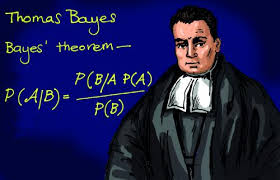
\includegraphics{img/README/portada.jpg}}{portada}}\label{portada}}

\pagebreak

\hypertarget{capuxedtulo-0-estructura-del-repositorio}{%
\section{Capítulo 0 Estructura del
repositorio}\label{capuxedtulo-0-estructura-del-repositorio}}

\begin{figure}
\centering
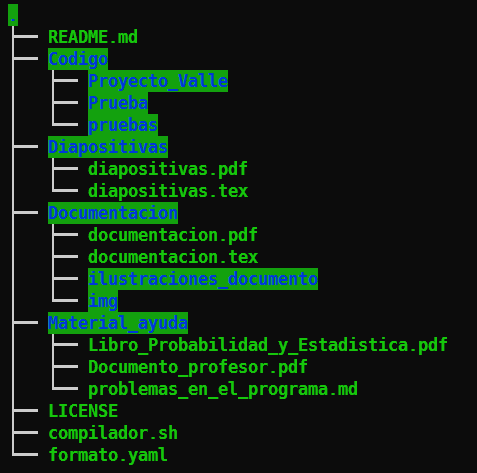
\includegraphics[width=3.125in,height=\textheight]{img/README/estructura.png}
\caption{estructura}
\end{figure}

Aquí mostramos la estructura de los archivos contenidos en el
repositorio para que puedas navegar dentro.

\hypertarget{cuxf3digo}{%
\subsection{Código}\label{cuxf3digo}}

Aquí se encuentra el código en \texttt{C++} y el \texttt{.exe} para
poder ejecutarlo, esta compilado para maquina de \texttt{64\ bits} en
sistema Windows pero esta el código disponible para su compilación.

\hypertarget{diapositivas}{%
\subsection{Diapositivas}\label{diapositivas}}

Sólo se encuentra el PDF de las diapositivas y el código \texttt{.tex}.

\hypertarget{documentaciuxf3n}{%
\subsection{Documentación}\label{documentaciuxf3n}}

Se encuentra una documentación del programa escrito en C++ y por tanto
es posible exportar un \texttt{.html} que explica todas las funcioens

\hypertarget{material-de-ayuda}{%
\subsection{Material de ayuda}\label{material-de-ayuda}}

Aquí se recopila, pdf´s dados por el profesor y externos con los cuales
se basó para crear el proyecto, se acumulan aquí, ya que la duración de
un archivo en la red tiene un tiempo limitado de vida y es posible que
si se desea mejorar este proyecto a futuro o hacerle un fork, sería
buena idea contar con el.

\hypertarget{archivos}{%
\subsection{Archivos}\label{archivos}}

\begin{itemize}
\tightlist
\item
  License (Licencia) la linecia es GNU.
\item
  README.md Es el mismo archivo que esta leyendo, solo que en formato
  \texttt{.md} para poder leerlo desde Github.
\end{itemize}

\hypertarget{capuxedtulo-1-introducciuxf3n}{%
\section{Capítulo 1 Introducción}\label{capuxedtulo-1-introducciuxf3n}}

La probabilidad es una rama de las matemáticas surgido en 1553 de la
mano de Gerolamo Cardano (1501-1576). Por otra parte
\textless\textless{} Pierre Fermat (1601-1665) y Blaise Pascal
(1623-1662) son conocidos como los padres de la teoría de la
probabilidad debido las grandes aportaciones que realizaron sobre este
campo\textgreater\textgreater{}

\textless\textless Andréi Kolmogorov. Fue el creador de la obra «Los
fundamentos de la Teoría de la Probabilidad» en la que expuso la
axiomática de Kolmogorov y le hizo ser reconocido como una eminencia de
la probabilidad\textgreater\textgreater.

La probabilidad busca encontrar el nivel de certeza de que ocurra un
evento dado, por lo cual existe un porcentaje asociado a ello, lo cual
puede ir desde un 0\% hasta un 100\%. Cuando el evento se aproxima a la
cantidad más alt, significa que es muy posible que suceda el evento, por
otro lado, cuando es cercano a 0 significa que es probable que el evento
no suceda.

Ahora un concepto más avanzado es el calculo de probabilidades dado por
un suceso anterior, es decir que tan probable es que suceda un evento
dado por que ocurra haya ocurrido otro evento. Para calcular dicha
probabilidad utilizamos el \textbf{teorema de Bayes} el cual nos
proporciona una forma fácil de calcular dicha probabilidad.

\hypertarget{conceptos}{%
\subsection{Conceptos}\label{conceptos}}

\textbf{Definición} (Regla de la adición).

\hspace{0pt}\\
\[
P(A \cup B) = P(A) + P(B) - P(A \cap B)
\]

\textbf{Definición 9 }(Probabilidad condicional) . La probabilidad
condicional de un evento \(B\) dado otro evento \(A\), escrita
\(P(B|A)\), se define \[
P(B|A)=\frac{P (A\cap B)}{P(A)}
\]

\textbf{Definición 13} (Clasificación Bayesiana). Considere el espacio
muestra compuesto por los siguientes vectores:

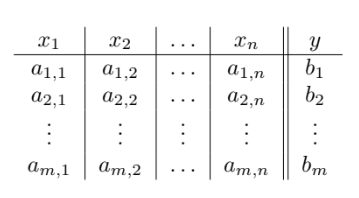
\includegraphics[width=3.125in,height=\textheight]{img/README/image-20220503051730015-16517649623251.png}

El modelo de clasificación Bayesiana se define como sigue: \[
\hat{y}=\max \left\{P\left(y_{i}\right) P\left(x_{1} \mid y_{i}\right) P\left(x_{2} \mid y_{i}\right) \ldots P\left(x_{n} \mid y_{i}\right) \mid i=1, \ldots, m\right\}
\]

\hypertarget{problema}{%
\subsection{Problema}\label{problema}}

Entrada: un espacio muestra, nuevos datos para clasificar.

Salida: la clasificación de los datos.

Dado un vector de condiciones \(\vec{Q}\) que contiene los valores
\([q_1,q_2,...,q_j]\) para \(j\) condiciones, a los cuales debe
igualarse \(Am_i\), obtener \(Y_{max}(\vec{Q})\) que es la probabilidad
más grande para dicho vector.

\textbf{Ejemplo.} Considere la siguiente base de datos.

\begin{longtable}[]{@{}llll@{}}
\toprule
\# & Usuario & Género & Calificación\tabularnewline
\midrule
\endhead
1 & F & Terror & 1\tabularnewline
2 & M & Acción & 3\tabularnewline
3 & F & Drama & 2\tabularnewline
4 & M & Drama & 2\tabularnewline
5 & F & Acción & 2\tabularnewline
6 & M & Terror & 3\tabularnewline
7 & F & Terror & 3\tabularnewline
8 & M & Drama & 1\tabularnewline
9 & F & Acción & 2\tabularnewline
\bottomrule
\end{longtable}

Calcule la calificación que le pondría un usuario \(M\) a una película
de Drama. \[
\begin{aligned}
&P(1) P(\mathrm{M} \mid 1) P(\text { Drama } \mid 1)=2 / 9 * 1 / 2 * 1 / 2=1 / 18 \\
&P(2) P(\mathrm{M} \mid 2) P(\text { Drama } \mid 2)=4 / 9 * 1 / 4 * 1 / 2=1 / 18 \\
&P(3) P(\mathrm{M} \mid 3) P(\text { Drama } \mid 3)=1 / 3 * 2 / 3 * 0=0
\end{aligned}
\] En este caso \(Y_{max}(\vec{Q})=1/18\), ya que es la mayor
probabilidad, con las condiciones que se le dieron.

\hypertarget{capuxedtulo-2-desarrollo}{%
\section{Capítulo 2 Desarrollo}\label{capuxedtulo-2-desarrollo}}

\hypertarget{soluciuxf3n}{%
\subsection{Solución}\label{soluciuxf3n}}

\hypertarget{pseudocuxf3digo}{%
\subsubsection{Pseudocódigo}\label{pseudocuxf3digo}}

\begin{Shaded}
\begin{Highlighting}[]
\NormalTok{inicio main():}
\NormalTok{    Datos}\OperatorTok{=}\NormalTok{ cargarDatos(nombre)}

\NormalTok{    Condiciones }\OperatorTok{\textless{}=} \BuiltInTok{input}\NormalTok{()}
\NormalTok{    Cuestion    }\OperatorTok{\textless{}=} \BuiltInTok{input}\NormalTok{()}

\NormalTok{    real    probabilidad }\OperatorTok{=} \FloatTok{1.0}\NormalTok{, masProbable }\OperatorTok{=} \FloatTok{0.0}
\NormalTok{    cadena  Argumento }\OperatorTok{=} \StringTok{"No hay coincidencias"}\NormalTok{, Objetivo, Regla }

\NormalTok{    por\_cada Objetivo en obten\_coleccion(Cuestion) realiza:}

\NormalTok{        probabilidad }\OperatorTok{=}\NormalTok{ obten\_Probabilidad(Datos,Objetivo)}

\NormalTok{        por\_cada Regla en obten\_coleccion(Condiciones) realiza:}

\NormalTok{            probabilidad }\OperatorTok{=}\NormalTok{ probabilidad }\OperatorTok{*}\NormalTok{ obten\_Probabilidad(Datos,Objetivo,Regla)}

\NormalTok{        fin\_bucle}

\NormalTok{        si (probabilidad }\OperatorTok{\textgreater{}}\NormalTok{ masProbable) entonces:}

\NormalTok{            mas probable }\OperatorTok{\textless{}=}\NormalTok{ probabilidad}
\NormalTok{            Argumento    }\OperatorTok{\textless{}=}\NormalTok{ Objetivo}

\NormalTok{        fin\_condicion}

\NormalTok{    fin\_bucle}

\NormalTok{    imprimir(Argumento)}

\NormalTok{fin\_main}

\NormalTok{inicio obten\_Probabilidad(Datos,Objetivo):}
\NormalTok{    retorna veces\_En\_Categoria(Datos,Objetivo) }\OperatorTok{/}\NormalTok{ (Datos.Altura }\OperatorTok{{-}} \DecValTok{1}\NormalTok{)}
\NormalTok{fin\_obten\_Probabilidad}

\NormalTok{inicio obten\_Probabilidad(Datos,Objetivo,Regla):}
\NormalTok{    retorna coincidencia(Datos,Objetivo,Regla) }\OperatorTok{/}\NormalTok{ veces\_En\_Categoria(Datos,Objetivo)}
\NormalTok{fin\_obten\_Probabilidad}
\end{Highlighting}
\end{Shaded}

\hypertarget{experimentos}{%
\subsection{Experimentos}\label{experimentos}}

Por cada nivel de dificultad usaremos un conjunto de datos (data-set) y
el problema cambiará de lo que se esta preguntado, en este caso serán 3
preguntas diferentes acerca de la probabilidad.

\end{document}
